
\documentclass[../notes.tex]{subfiles}

\graphicspath{{\subfix{../img/}}}

\begin{document}

\part{ECE444: Software Engineering}

\marginnote{Taught by Prof. Shurui Zhou}
\section{Preliminary}
\subsection{Lecture 1, 2}
\begin{itemize}
	\item Software engineering is different from what coding is; design, architecture, documentation, testing, etc v.s. just script kiddie-ing
	\item \href{https://en.wikipedia.org/wiki/Vasa_syndrome}{Vasa syndrome}
	\item Rockstar engineers are a myth
\end{itemize}

\section{Project Management}
\subsection{Lecture 3}

\begin{definition}
	\href{https://en.wikipedia.org/wiki/Conway%27s_law}{Conway's law} states that 'Any organization that designs a system (defined broadly) will produce a design whose structure is a copy of the organization's communication structure`.
\end{definition}


The waterfall method is slow and costly and defects can be extremely costly, especially early on in the development lifecycle.

\begin{figure}[H]
	\centering
	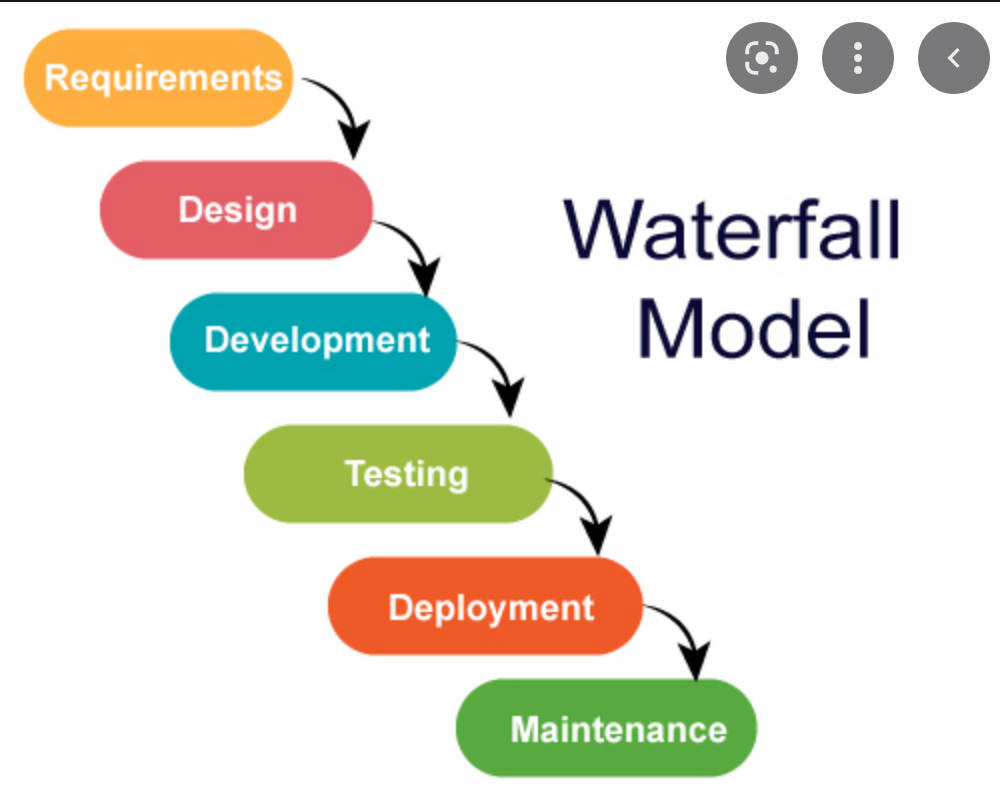
\includegraphics[width=0.8\linewidth]{img/image_2022-09-14-14-35-07.png}
	\caption{Waterfall method}
\end{figure}

In order to address this the V model was introduced which increases the amount of testing to reduce the possibility of having to rework everything
\begin{figure}[H]
	\centering
	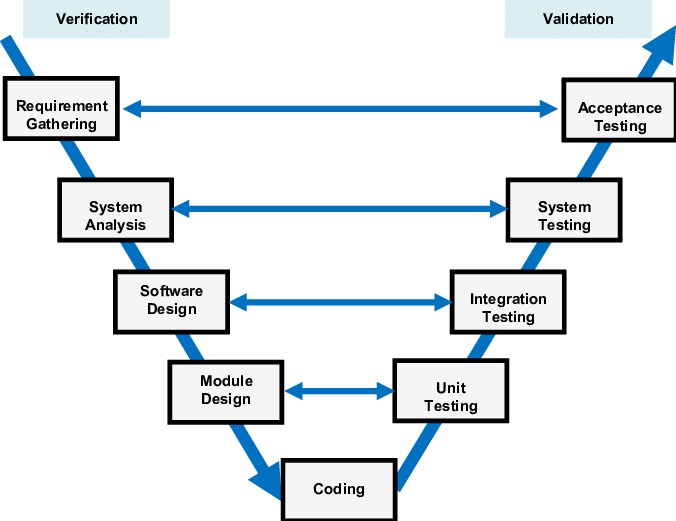
\includegraphics[width=0.8\linewidth]{img/image_2022-09-14-14-36-18.png}
	\caption{V model}
\end{figure}

Generally speaking the waterfall model isn't used much anymore due to the reality that software specifications change on a near daily basis.\marginnote{Recall: aUToronto Spring 2022 integration hell}


\subsubsection{Agile}

Agile is a project management approach which, in most general terms, seeks to respond to change and unpredictability using incremental, iterative work (sprints).
This allows for a balance between the need for predictability and the need for flexibility.
Some agile methods include:
\begin{itemize}
	\item Extreme programming: really really fast iteration (think days)
	\item Scrum: 2-4 week sprints with standups and backlogs; sticky notes for tasks, etc. Think kanban boards. Daily scrum meetings to unblock ASAP. Development lifecycle is therefore a series of sprints.
	\item On-site customer; frequent interaction with end users to figure out what exactly they need.
\end{itemize}


\subsection{I dropped this course}
\textbf{I decided to drop this course because the courseload was a little too much to handle between EngSci ECE, clubs, design teams, work, and trying to have a life.} 

\end{document}

